% !TEX root = ../main.tex
\chapter{Solution}
\label{chap:solution}

Even though the changes introduced to Rust on \fref{subsec:rfc2000} add the
necessary syntax to abstract code over constant expressions, Rust lacks of a
mechanism to reason deeply about constant expressions. As a consequence is not
possible to typecheck or provide any compile time guarantees over the safety of
using generics over constant values.  On this chapter, we introduce
\textsc{sire}, a symbolic evaluator for Rust, this provides a foundation to
treat function equality via an SMT solver. 

Symbolic execution evaluates a program in an abstract manner, taking symbols
representing each program's input, instead of concrete values, and then
executing the program propagating with each symbol. With a symbolic representation
of a function is possible to reason deeply about its behaviour, in particular
is possible to decide if two functions evaluate to the same values for every
possible input or which input for a function would produce a particular result or failure.

With this taken into account, is possible to extend Rust's compiler to reason
about generic types over constant values in a similar manner to its generics
over types counterpart, providing trait resolution and type
inference for this new kind of generics.

The remaining part of this section explains the inner processes done by
\textsc{sir} and proposes a solution to the problems stated in
\Fref{chap:motivation}.

\section{Symbolic execution of Rust programs}
\label{sec:symbolic_execution}

\textsc{sire} is a symbolic executor for the \textsc{mir} of Rust, which is
able to interact with the Rust's compiler. After the compiler generates the
\textsc{mir} for a function, \textsc{sire} takes this representation and
evaluates it into an small symbolic intermediate representation or \textsc{sir}
for short.

Currently \textsc{sire} can only evaluate an small subset of all possible
\textsc{mir} functions. Specifically, it can evaluate functions without mutable
arguments nor mutable references as arguments containing the following subset
of \textsc{mir}:

\begin{itemize}
    \item Statements: \inrust{Assign}, \inrust{StorageLive} and \inrust{StorageDead}.
    \item Terminators: \inrust{Goto}, \inrust{Return}, \inrust{Call} and \inrust{SwitchInt}.
    \item Rvalues: \inrust{BinaryOp}, \inrust{Ref} and \inrust{Use}.
    \item Operands: \inrust{Move}, \inrust{Copy} and \inrust{Constant}.
\end{itemize}

In addition, \textsc{sire} only supports integer and boolean types. Support for
structures, tuples, enumerations and arrays is planned for future work.
Floating point types are not supported given that they lack of a total equality
relation. \footnote{A deeper discussion about the different notions of equality
can be found on
\href{https://github.com/rust-lang/rfcs/blob/master/text/1445-restrict-constants-in-patterns.md}{RFC-1445}.}

\textsc{sire} has an store to read and write symbolic expressions during
evaluation. The symbolic execution of a function starts by allocating each of
the function's arguments as symbols into its store, then each \textsc{mir}
expression is evaluated into a \textsc{sir} expression. When the return
statement of the \textsc{mir} of the function is reached, \textsc{sire} takes
the symbolic expression corresponding to the return value of the function from
its store and returns it, providing a symbolic representation of the function. 

\begin{figure}[h]
    \centering
    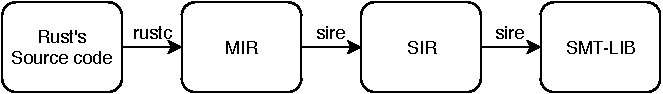
\includegraphics[width=15cm]{images/flow.pdf}
    \caption{The different transformation stages of a constant function}
    \label{fig:flow}
\end{figure}


\subsection{Symbolic intermediate representation}

\textsc{sir} is a relatively simple language. Functions are the main construct
of \textsc{sir} and function arguments are numbered following the same
convention as \textsc{mir} where the zeroth argument is the return place. The
grammar for \textsc{sir} can be found on \Fref{lst:sir_grammar}.

\begin{listing}[H]
    \begin{minted}{ebnf}
    defun   = '(defun' name {ty} expr ')';
    expr    = value | '('expr {expr}')' | '('op expr expr')' | 
             '(switch' expr {'('expr '->' expr')'} defcase);
    value   = '_'num | '(const' ty num')' | name;
    defcase = '(else ->' expr')';
    ty      = '(int' num')' | '(uint' num')' | 'bool';
    num     = ? a positive integer ?;
    name    = ? an string denoting the name of a function ?;
    op      = ? a binary operator ?;
    \end{minted}
    \caption{\textsc{sir}'s grammar in EBNF}
  \label{lst:sir_grammar}
\end{listing}

The body of each function is composed of expressions which can be function
applications, binary operations, switch statements or pure values. 

There are only three kinds of values: Function arguments, constants and
function names. Constants are stored as raw bits with its corresponding type. 

Finally, switch statements are composed by the value to be compared, the
possible values that it can take, and the result for each possible value (there
must be always a default result). 

\begin{table}[H]
    \centering
    \begin{tabular}{ | c | c | }
        \hline
        \inrust{StatementKind} variant & Effect \\
        \hline
        \inrust{Assign(place, rvalue)} & Evaluate \inrust{rvalue} and store it into \inrust{place} \\
        \hline
        \inrust{StorageLive(local)} & Add the key \inrust{local} into the store \\
        \hline
        \inrust{StorageDead(local)} & Remove the key \inrust{local} from the store \\
        \hline
    \end{tabular}
    \caption{Evaluation of each \textsc{mir} statement and the effect it has into \textsc{sire}'s store.}
  \label{tab:sire_statements}
\end{table}

\begin{table}[H]
    \centering
    \begin{tabular}{ | c | c | }
        \hline
        \inrust{Operand} variant & Result \\
        \hline
        \inrust{Move(place)} & Return the value stored in \inrust{place} \\
        \hline
        \inrust{Copy(place)} & Return the value stored in \inrust{place} \\
        \hline
        \inrust{Constant(constant)} & \makecell{Extract the bits of  \inrust{constant} and returns a \textsc{sir}\\ constant with the corresponding type} \\
        \hline
    \end{tabular}
    \caption{Result of the evaluation done by \textsc{sire} for each \inrust{Operand} variant.}
    \label{tab:sire_operand}
\end{table}

\begin{table}[H]
    \centering
    \begin{tabular}{ | c | c | }
        \hline
        \inrust{Rvalue} variant & Result \\
        \hline
        \inrust{BinaryOp(bin_op, op1, op2)} & \makecell{Evaluate \inrust{op1} and \inrust{op2}, and build the\\ corresponding \textsc{sir} binary operation\\ using \inrust{bin_op}} \\
        \hline
        \inrust{Rvalue::Ref(_, Shared, place)} & Return the value stored in \inrust{place}\\
        \hline
        \inrust{Use(operand)} & Evaluate \inrust{operand}\\
        \hline
    \end{tabular}
    \caption{Result of the evaluation done by \textsc{sire} for each possible \inrust{Rvalue} variant.}
    \label{tab:sire_rvalue}
\end{table}

\begin{table}[H]
    \centering
    \begin{tabular}{ | c | c | }
        \hline
        \inrust{TerminatorKind} variant & Effect \\
        \hline
        \inrust{Return} & Stop execution \\
        \hline
        \inrust{Goto{target}} & \makecell{Continue execution into \\ the \inrust{target} block} \\
        \hline
    \inrust{Call{func, args, destination}} & \makecell{Evaluate \inrust{func} and \inrust{args}, store them\\ in the place stated in \inrust{destination}.\\ Continue the execution as stated in\\ \inrust{destination}} \\

        \hline
        \inrust{SwitchInt{discr, values, targets}} & \makecell{Fork execution for each block in\\ \inrust{targets} replacing \inrust{discr} by the\\ corresponding value in \inrust{values}} \\
        \hline
    \end{tabular}
    \caption{Evaluation of each \textsc{mir} terminator and the effect it has into \textsc{sire}'s execution flow.}
  \label{tab:sire_terminator}
\end{table}

The evaluation done by \textsc{sire} for each one of the \textsc{mir}
expressions mentioned on section \fref{sec:symbolic_execution} is explained
on Tables \ref{tab:sire_statements}-\ref{tab:sire_terminator}.

As an example, when executing the code on \Fref{lst:rust_sire_example}, the
\textsc{mir} and \textsc{sir} generated can be found on \Fref{fig:mir_sire_example} and \Fref{lst:sir_sire_example} respectively. Even
though the code on \Fref{lst:rust_sire_example} is similar to the one found on
\Fref{lst:sir_sire_example}, \textsc{sire} is executing each instruction of
\Fref{fig:mir_sire_example} to generate this representation.

\begin{listing}[H]
    \begin{minted}{rust}
    fn distance(x: i32, y: i32) -> i32 {
        if x > y {
           x - y
        } else {
           y - x
        }
    }
    \end{minted}
    \caption{A simple Rust function to be evaluated using \textsc{sire}}
  \label{lst:rust_sire_example}
\end{listing}


\begin{figure}[h]
    \centering
    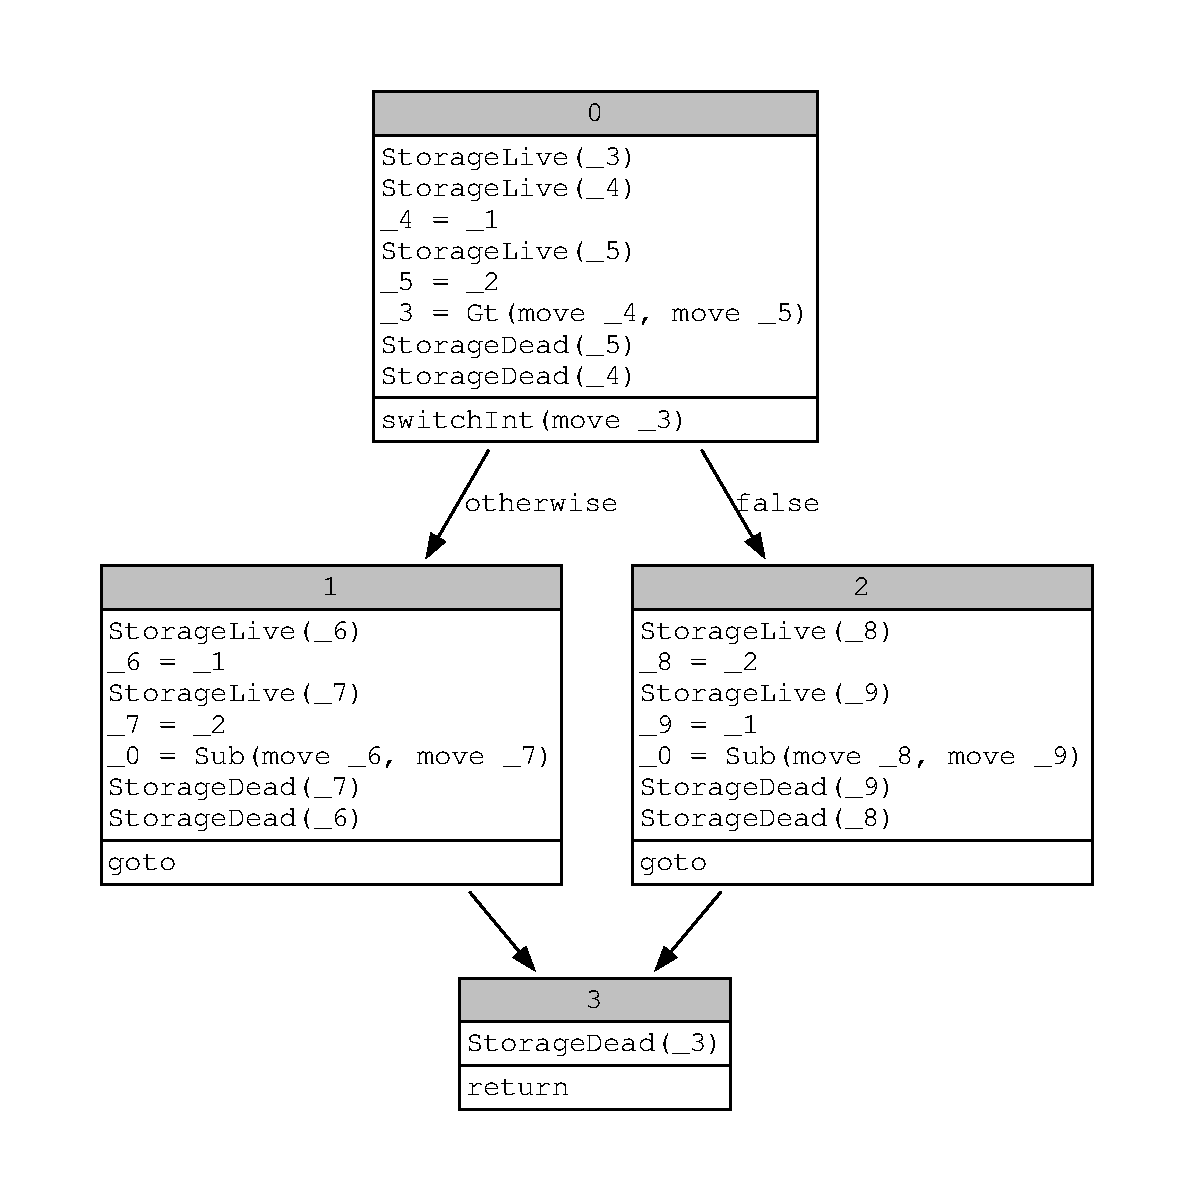
\includegraphics[height=12cm]{images/distance.pdf}
    \caption{The \textsc{mir} of the \inrust{distance} function on \Fref{lst:rust_sire_example}}
    \label{fig:mir_sire_example}
\end{figure}

\begin{listing}[H]
    \begin{minted}{lisp}
    (defun distance (int 32) (int 32) (int 32) 
        (switch (> _1 _2) 
            ((const bool 0) -> (- _2 _1)) 
             (else -> (- _1 _2))))
    \end{minted}
    \caption{The \textsc{sir} of the \inrust{distance} function on \Fref{lst:rust_sire_example}}
  \label{lst:sir_sire_example}
\end{listing}

\begin{listing}[H]
    \begin{minted}{lisp}
    (define-fun distance 
     ((x1 (_ BitVec 32)) (x2 (_ BitVec 32))) (_ BitVec 32) 
     (ite (bvsgt x1 x2) (bvsub x1 x2) (bvsub x2 x1)))
    \end{minted}
    \caption{The \textsc{smt-lib} snippet for the \textsc{sir} of the \inrust{distance} function on \Fref{lst:rust_sire_example}}
  \label{lst:smt_sire_example}
\end{listing}

\subsection{Equality of symbolic functions}

Two \textsc{sir} functions are considered equal if they have the same type and
evaluate to the same expression for every possible argument. For simple
arithmetic expressions, this could be achieved via E-unification. However,
\textsc{sir} functions contain control flow operations and recursive calls, in
this case a theorem prover such as Z3 is up to the task. \textsc{sire} can
transform every \textsc{sir} function into an small snippet in the
\textsc{smt-lib} format to use it in an SMT solver.

\begin{listing}[h]
    \begin{minted}{rust}
    fn alt_dist(x: i32, y: i32) -> i32 {
        let sign: i32; 
        if x > y {
           sign = 1;
        } else {
           sign = -1;
        }
        sign * (x - y)
    }
    \end{minted}
    \caption{An alternative implementation of the \inrust{distance} function on \Fref{lst:rust_sire_example}}
  \label{lst:alt_distance}
\end{listing}

Integer types on \textsc{sir} are transformed into \textsc{smt-lib} bit vectors
of the corresponding length and the signed or unsigned arithmetic operations
are transformed according to the type of the operands. Switch expressions are
transformed into nested conditionals, preserving the order of the switch
expression's branches. An example of such snippets can be found on
\Fref{lst:smt_sire_example}. 

To decide if two functions are equal, is enough to write an small
\textsc{smt-lib} snippet checking if the two functions are equal in their whole
range. On \Fref{lst:func_equality}, the \inrust{distance} function is compared
with an alternative implementation found on \Fref{lst:alt_distance}. 

It is important to consider that the SMT solver might find no answer to one of
this queries under time constrains. This is because in the worst case scenario,
some SMT solvers will try to check every possible output to decide if two
functions are equal. 

\begin{listing}[H]
    \begin{minted}{lisp}
    ;; Definition of distance provided by sire
    (define-fun distance 
     ((x1 (_ BitVec 32)) (x2 (_ BitVec 32))) (_ BitVec 32) 
     (ite (bvsgt x1 x2) (bvsub x1 x2) (bvsub x2 x1)))

    ;; Definition of alt_dist provided by sire
    (define-fun alt_dist 
     ((x1 (_ BitVec 32)) (x2 (_ BitVec 32))) (_ BitVec 32) 
     (ite (bvsgt x1 x2) 
      (bvmul (_ bv1 32) (bvsub x1 x2)) 
      (bvmul (_ bv4294967295 32) (bvsub x1 x2))))
    
    ;; Assert that the functions are equal
    (assert (forall ((x1 (_ BitVec 32)) (x2 (_ BitVec 32))) 
     (= (distance x1 x2) (alt_dist x1 x2)))) 

    ;; Check if the assertions can be satisfied
    (check-sat) ; sat
    \end{minted}
    \caption{Equality check between the \inrust{distance} and \inrust{alt_dist} functions}
  \label{lst:func_equality}
\end{listing}


\subsection{Type inference}

Type inference is the process of inferring the type of an expression, this is
what makes possible to write Rust code with almost no type annotations. The
Rust compiler does type inference by adding constrains over inference variables
and then trying to bind each variable to a concrete type.

The relevant constrains for this work are equality constrains, meaning that a
type variable must be equal to another. Subtyping constrains are not discussed
here, given that the subtyping relation is only relevant when dealing with
lifetimes.

When an equality constrain is added, and both the type variables correspond to
types with constants as generics parameters, this equality constrain over types
can be reduced over an equality constrain over its constant parameters, i.e.,
as a constrain of equality between functions, which can be represented and
solved using \textsc{sire}. 

Note that it is possible that an SMT solver is unable to decide if a clause is
satisfiable or not. For example, is possible to encode a root finding problem
as a function equality problem, these kind of problems do not have an analytic
solution for high degree polynomials.

As a consequence, is not possible to do type checking nor type inference for
every program with generics over constant values using symbolic execution.

\section{Bounds for generics over constants}

As explained on \Fref{sec:traits}, Rust's generic type parameters can be
constrained indicating that the type parameters must implement an specific
trait. Extending this behavior to constant parameters would allow the user to
constrain constant expressions using predicates over them, an example of this
can be seen on \Fref{lst:head_const_generics}, where the \inrust{head}
function's constant parameter \inrust{N} is bounded to be strictly positive,
guaranteeing that the first element of the array always exists. 

\begin{listing}[h]
	\begin{minted}{rust}
    fn head<T, const N: usize>(array: &[T; N]) -> &T
    where {N > 0} {
        &array[0]
    }
    \end{minted}
    \caption{Type-safe access to the first element of a non-empty array using bounded generics}
  \label{lst:head_const_generics}
\end{listing}

The difference between this implementation and a traditional one as in
\Fref{lst:head_no_bounds} is the stage in which the condition \inrust{N > 0} is
checked. When using the function provided in \Fref{lst:head_const_generics},
the condition is verified in compilation, during the monomorphization stage. On
the other case, the condition is verified also in compilation, during the
constant propagation stage, or in a case where the compiler is doing few
optimizations, the condition would be verified every time the function is
called during execution.

Using the \inrust{Option} type also introduces an small memory overhead, given
that enumerations require additional memory space to indicate which variant is
being used. This being said, using bounded generics over constants would
provide a more consistent and performant abstraction for providing type-safe
access to arrays.

\begin{listing}[h]
	\begin{minted}{rust}
    fn head<T, const N: usize>(array: &[T; N]) -> Option<&T> {
        if N > 0 {
            Some(&array[0])
        } else {
            None
        }
    }
    \end{minted}
    \caption{Type-safe access to the first element of a non-empty array using the \inrust{Option} type}
  \label{lst:head_no_bounds}
\end{listing}

In order to check conditionals during monomorphization, is necessary to
evaluate the conditionals in the desired constants.  For example, if the user
calls the \inrust{head} function in the \inrust{[1, 2, 3]} array, the compiler
must decide if \inrust{N > 0} is true when \inrust{N = 3} is true.  Both
\textsc{miri} and \textsc{sire} would be able to perform such task. In
particular, \textsc{sire} can generate the \textsc{sir} of \inrust{N > 0} and
use an SMT solver to check the conditional.

\section{Generic traits over constants}

The RFC-2000 allows the user to write implementations for traits which are
generic over constant values, solving the problem of implementing traits for
arrays of arbitrary size as shown in \Fref{lst:trait_const_generics}. However,
there is no mechanism to extend trait specialization for generics over constant
values. As a consequence, if a trait has several implementations for a single
type as in \Fref{lst:trait_const_generics_spec} is necessary to decide which
implementation will be used on each case. 

\begin{listing}[h]
	\begin{minted}{rust}
    impl<A: Sized, B, const N: usize> PartialEq<[B; N]> 
    for [A; N] where A: PartialEq<B> {
        fn eq(&self, other: &[B; N]) -> bool {
            self[..] == other[..]
        }
        fn ne(&self, other: &[B; N]) -> bool {
            self[..] != other[..]
        }
    }
	\end{minted}
    \caption{Implementing the \inrust{PartialEq} trait for all array sizes}
  \label{lst:trait_const_generics}
\end{listing}

\begin{listing}[h]
	\begin{minted}{rust}
    impl<const N: usize> PartialEq<[i32; N]> for [i32; N]
    with {N + 1 > 1} {
        ...
    }
   
    impl<const N: usize> PartialEq<[i32; N]> for [i32; N]
    with {N > 0} {
        ...
    }
	\end{minted}
    \caption{Two implementations of a trait for the same type}
  \label{lst:trait_const_generics_spec}
\end{listing}

The basic strategy to decide which implementation to use is based on the notion
of specificity: If there is more than one implementation of a trait for the
same type, the compiler will give priority to the one which is more specific.
\footnote{More information about trait specialization can be found at
\href{https://github.com/rust-lang/rfcs/blob/master/text/1210-impl-specialization.md}{RFC-1210}.}

When generics are taken into account, this means that an implementation with
boundless generics is less specific that one with bounded generics. At the same
time, an implementation with bounded generics is more specific than one without
bounds. Finally, when two implementations have bounded generics, the
specificity degree will be decided by the specificity of its bounds. One bound
is more specific than another if the first implies the second.

\begin{listing}[h]
	\begin{minted}{lisp}
        ;; Definition of bound_a provided by sire
        (define-fun bound_a
         ((x1 (_ BitVec 64))) Bool 
         (bvugt (bvadd x1 (_ bv1 64)) (_ bv1 64)))

        ;; Definition of bound_b provided by sire
        (define-fun bound_b 
         ((x1 (_ BitVec 64))) Bool 
         (bvugt x1 (_ bv0 64)))

        ;; Assert that the first bound implies the second
        (assert (forall ((x1 (_ BitVec 64))) 
         (implies (bound_a x1) (bound_b x1))))

        ;; Check if the assertions can be satisfied
        (check-sat) ; sat
	\end{minted}
    \caption{Checking if \inrust{N + 1 > 1} is more specific than \inrust{N > 0}.}
  \label{lst:trait_spec_smt}
\end{listing}

Naturally, an SMT solver is capable of checking if one predicate implies
another, meaning that we can take the \textsc{sir} of the bounds and decide if
one is more specific than another. To decide which implementation is more
specific in \Fref{lst:trait_const_generics_spec}, is enough to generate an
\textsc{smt-lib} snippet like the one found in \Fref{lst:trait_spec_smt}.

When the SMT solver is not able to decide which bound is more specific, the
same posture as in RFC-1210 can be taken and throw an error telling the user
that the implementations are overlapping.
